\documentclass[11pt,a4paper]{article}

\usepackage[T1]{fontenc}
\usepackage[utf8]{inputenc}
\usepackage{libertinus}
\usepackage[scaled=0.86]{beramono}
\usepackage{microtype}
\usepackage[margin=2.3cm]{geometry}
\usepackage{graphicx}
\usepackage{booktabs}
\usepackage{tabularx}
\usepackage{array}
\usepackage{multirow}
\usepackage[table]{xcolor}
\usepackage{enumitem}
\usepackage{caption}
\usepackage{float}
\usepackage{amsmath}
\usepackage{tikz}
\usetikzlibrary{arrows.meta,positioning,shapes.geometric,fit,backgrounds}
\usepackage{fancyhdr}
\usepackage{titlesec}
\usepackage{etoolbox}
\usepackage{hyperref}
% Every top-level topic starts on a new page.
\pretocmd{\section}{\clearpage}{}{}

\definecolor{aq}{HTML}{5242C4}
\definecolor{aqsoft}{HTML}{EBE8FB}
\definecolor{ink}{HTML}{171A2B}
\definecolor{muted}{HTML}{4B5064}
\definecolor{safe}{HTML}{1D7A52}
\definecolor{safesoft}{HTML}{E2F3EA}
\definecolor{warn}{HTML}{9A5800}

\hypersetup{colorlinks=true,linkcolor=aq,urlcolor=aq,citecolor=aq,
  pdftitle={AQoSE: Adaptive QoS Engine},pdfauthor={AQoSE team, Teliport Season 4}}
\graphicspath{{../charts/}}
\captionsetup{font=small,labelfont={bf,color=aq},format=plain}
\setlist{itemsep=2pt,topsep=4pt}
\titleformat{\section}{\Large\bfseries\color{ink}}{\color{aq}\thesection}{0.8em}{}
\titleformat{\subsection}{\large\bfseries\color{ink}}{\color{aq}\thesubsection}{0.8em}{}
\titleformat{\paragraph}[runin]{\bfseries\color{ink}}{}{}{}[.]
\pagestyle{fancy}\fancyhf{}
\fancyhead[L]{\small\color{muted}AQoSE: Adaptive QoS Engine}
\fancyhead[R]{\small\color{muted}Teliport Season 4 $\cdot$ Tata Elxsi}
\fancyfoot[C]{\small\thepage}
\renewcommand{\headrulewidth}{0.3pt}
\setlength{\parskip}{0.45em}\setlength{\parindent}{0pt}
\newcommand{\num}[1]{\mbox{#1}}
\newcommand{\ours}[1]{\textbf{\color{aq}#1}}

\begin{document}

\begin{titlepage}
\vspace*{2.2cm}
{\color{aq}\rule{\linewidth}{1.2pt}}\par\vspace{0.6cm}
{\fontsize{40}{44}\selectfont\bfseries\color{ink} AQoSE}\par\vspace{0.3cm}
{\LARGE\color{ink} Adaptive QoS Engine}\par\vspace{0.4cm}
{\large\color{muted} A predictive traffic classifier that tells Linux CAKE\\ which connection is the call or the game}\par
\vspace{0.6cm}{\color{aq}\rule{\linewidth}{1.2pt}}\par
\vspace{1.2cm}
{\large Full project report}\par\vspace{0.2cm}
{\color{muted} Tata Elxsi Teliport, Season 4\\ Team: [team member names]\\ October 16, 2026}
\vfill
\begin{minipage}{\linewidth}\small\color{muted}
Every number in this report was measured in emulation, on one laptop (Fedora 43, Linux 7.2.8, 12th-gen Intel Core i5, 16 threads), in a rootless network-namespace testbed. The system has not yet run on a real router or in a real home. Source, results and every script that produced them are in the project repository.
\end{minipage}
\end{titlepage}

\section*{Summary}
\addcontentsline{toc}{section}{Summary}

Home routers that run CAKE, the strongest open-source queue manager, already keep most calls and games smooth: CAKE shares the line fairly between devices and then between each device's connections. It fails in one common situation: \emph{a call or a game on a device that is also downloading, uploading or sharing files}. Fairness then gives the call a small slice of its own device's share, and nothing tells CAKE which connection is the call. Existing tools sort traffic with fixed thresholds (``many packets per second means bulk''), which mistake video calls and cloud games for downloads because they also send many packets.

AQoSE is an add-on to CAKE. It watches the sizes and timing of the first eight packets of each new connection (headers only, never content), predicts the kind of traffic with a small gradient-boosted tree model, picks the CAKE priority tin with the lowest expected damage, and writes that choice as a connection label CAKE reads for every packet. A safety shield checks every change, a verifier undoes changes that raise delay, and a separate watchdog returns the router to plain CAKE within about two seconds if AQoSE stops.

\begin{table}[H]\centering\small
\begin{tabular}{@{}lrrrr@{}}
\toprule
Late video or game frames (median of 10 seeds) & Plain CAKE & cake-autorate & Threshold rules & \textbf{AQoSE} \\
\midrule
S6 HD call on a laptop that is sharing files & 94.3\% & -- & 94.4\% & \ours{0.6\%} \\
S5 work call on a busy evening, backup running & 93.3\% & 93.3\% & 78.7\% & \ours{0.1\%} \\
S7 cloud game on a PC fetching an update & 83.2\% & -- & 19.4\% & \ours{1.0\%} \\
S2 line drops to a fifth of its speed & 55.5\% & 4.6\% & 55.6\% & \ours{0.9\%} \\
S12 a real WhatsApp video call, replayed (5 seeds) & 57.0\% & -- & 42.7\% & \ours{2.4\%} \\
\bottomrule
\end{tabular}
\end{table}

\begin{itemize}
\item \textbf{Against plain CAKE}, over every seed-paired run of the frozen system: better in 49, tied in 41, worse in 0 (seeds 0--9); better in 21, tied in 29, worse in 0 on fresh seeds never used in development.
\item \textbf{Against the threshold rules} existing tools use: never worse in any run (52 better and 38 tied on seeds 0--9).
\item \textbf{Against cake-autorate}, the community tool for changing line speed: better in 20 of 20 runs.
\item \textbf{Real traffic.} Replayed real WhatsApp video calls were recognised as video calls within 0.13 s in all 20 runs and kept in the Video tin; late frames fell from 57\% to 2.4\% and from 79\% to 14\%.
\item \textbf{Sealed test set}, opened once: accuracy 0.969 and macro-F1 0.73 on 1,213 flows from 183 unseen sessions; no video call or cloud-gaming flow sent to Bulk (qosify's defaults: 14\% and 78\%).
\item \textbf{Cost}: the controller uses about 3.6\% of one laptop core; classifying one connection takes about 6\,\textmu s in Go.
\end{itemize}

The defensible claim is narrower than ``beats CAKE'' and sharper: \textbf{AQoSE beats plain CAKE when a call or a game shares its device with heavy traffic, and when the line's speed changes; elsewhere it ties CAKE, and it never did worse than threshold rules.} Section~\ref{sec:limits} lists what these results do not show.

\clearpage
\tableofcontents

%======================================================================
\section{The problem}

\paragraph{What CAKE already does well} CAKE (Common Applications Kept Enhanced) shapes traffic just below the line rate so that queues build in the router, where they can be managed, and not in the modem's oversized buffer. It shares the link fairly between hosts, then between each host's flows. In our testbed this alone takes a call's late frames from 77\% (no queue management) to 0\% whenever the call is alone on its device (scenarios S1, S4, S10).

\paragraph{Where it fails} Fairness protects a call from \emph{other} devices, not from its own. A laptop on an HD video call that is also running a file-sharing client with twenty connections gives the call one twenty-first of its share. In scenario S6 that leaves 94\% of the call's frames late. The same happens to a cloud game on a PC fetching a game update (S7, 83\% late).

\paragraph{Why tins are not used today} CAKE's \texttt{diffserv4} mode has four priority tins: Voice, Video, Best Effort and Bulk. Something must decide which flow belongs in which. Applications rarely set priority marks that survive the internet, and the tools that sort traffic on home routers (qosify on OpenWrt, for example) use thresholds on packet rate and size. An HD video call sends 400--600 packets a second and a cloud game over 1,000, so those rules call both ``bulk''. On our sealed test set, qosify's default rules sent 78\% of cloud-gaming flows and 14\% of video-call flows to Bulk.

%======================================================================
\section{Design}

\subsection{Principle: no AQoSE code on the per-packet path}

The kernel forwards every packet and CAKE queues it. AQoSE writes one label per connection into the kernel's connection tracker (conntrack), and CAKE reads that label for each packet. If AQoSE is slow, wrong or dead, packets still flow; an unlabelled connection is exactly plain CAKE. Figure~\ref{fig:flow} follows one connection from start to end.

\begin{figure}[H]\centering
\begin{tikzpicture}[
  node distance=0.42cm,
  every node/.style={font=\small},
  box/.style={draw=aq,rounded corners=2pt,fill=white,text width=8.6cm,align=center,inner sep=4pt,minimum height=0.85cm},
  ends/.style={draw=aq,fill=aq,text=white,rounded corners=10pt,text width=6cm,align=center,inner sep=5pt,font=\small\bfseries},
  check/.style={draw=aq,fill=aqsoft,diamond,aspect=3.2,align=center,inner sep=1pt,text width=3.4cm},
  safe/.style={draw=safe,fill=safesoft,rounded corners=2pt,text width=2.9cm,align=center,inner sep=4pt},
  arr/.style={-{Stealth[length=2.2mm]},thick,color=ink},
  exitarr/.style={-{Stealth[length=2.2mm]},thick,dashed,color=safe}]
\node[ends] (start) {START: a device opens a connection};
\node[box,below=of start] (k1) {\textbf{1} Kernel creates a conntrack entry, mark 0: plain CAKE for now};
\node[box,below=of k1] (k2) {\textbf{2} Extractor receives packets 1--8, headers only (nflog)};
\node[box,below=of k2] (k3) {\textbf{3} Classifier: 259 trees, $\approx$6\,\textmu s, odds for 7 classes};
\node[box,below=of k3] (k4) {\textbf{4} Decision engine: lowest expected damage, then guards $\rightarrow$ tin};
\node[check,below=of k4] (k5) {\textbf{5} Safety shield:\\ within every limit?};
\node[box,below=of k5] (k6) {\textbf{6} Enforcer writes the conntrack mark and reads it back};
\node[box,below=of k6] (k7) {\textbf{7} CAKE queues every packet of the flow in its tin, both directions};
\node[check,below=of k7] (k8) {\textbf{8} Each second:\\ still like its class?};
\node[ends,below=of k8] (end) {END: connection closes};
\node[safe,right=1.1cm of k5] (plain) {Stays in plain CAKE};
\draw[arr] (start)--(k1); \draw[arr] (k1)--(k2); \draw[arr] (k2)--(k3); \draw[arr] (k3)--(k4);
\draw[arr] (k4)--(k5); \draw[arr] (k5)--node[right,font=\scriptsize]{accept}(k6); \draw[arr] (k6)--(k7);
\draw[arr] (k7)--(k8); \draw[arr] (k8)--node[right,font=\scriptsize]{connection ends}(end);
\draw[arr] (k8.west) -| ([xshift=-7mm]k3.west) node[pos=0.75,left,font=\scriptsize,align=right]{changed:\\ ask again} -- (k3.west);
\draw[exitarr] (k5.east)--node[above,font=\scriptsize]{reject}(plain.west);
\draw[exitarr] (k3.east) -| node[pos=0.75,right,font=\scriptsize]{timeout or error}(plain.north);
\draw[exitarr] (k6.east) -| node[pos=0.75,right,font=\scriptsize]{mismatch: undo}(plain.south);
\end{tikzpicture}
\caption{Life of one connection. Solid arrows are the main path; dashed arrows are the ways out, and every one ends in plain CAKE. Alongside run a capacity estimator (every 100 ms), a QoE verifier (after each promotion) and a watchdog (every 250 ms); their proposals pass through the same shield.}
\label{fig:flow}
\end{figure}

\subsection{Components}

\begin{table}[H]\centering\small
\begin{tabularx}{\linewidth}{@{}l>{\raggedright\arraybackslash}X@{}}
\toprule
Process & Role \\
\midrule
\texttt{aqosd} (Go) & The controller: feature extractor, flow table, reclassifier, capacity estimator, verifier, lease API, safety shield, enforcer, heartbeat \\
\texttt{aqos-classify} (Go) & The model and decision rule behind a Unix socket, one JSON object per line \\
\texttt{aqos-watchdog} (Go, standard library only) & Restores plain CAKE when the heartbeat stops \\
\texttt{aqos\_ml} (Python) & Training, the threshold rules (B4), traffic generators, experiment runner, statistics \\
\texttt{aqos-testbed} (Go) & Builds the emulated home from network namespaces, rootless \\
\bottomrule
\end{tabularx}
\end{table}

\paragraph{Marking} The label is the low three bits of the conntrack mark; CAKE's \texttt{fwmark 0x7} option maps mark $n$ to tin $n$ (1 Bulk, 2 Best Effort, 3 Video, 4 Voice). On upload a postrouting rule copies the label to each packet; on download, packets are redirected to an IFB device whose filter restores it (\texttt{ctinfo cpmark 0x7}) before a second CAKE instance. Mark 0 falls through to CAKE's own DSCP handling, so ``unlabelled equals plain CAKE'' holds by construction, and removing two rules turns the whole system off. Verified in the testbed for both directions, IPv4 and IPv6.

\paragraph{Feature extractor} One nftables rule, \texttt{ct packets < 9 log group 5 snaplen 64}, sends the first eight packets of every flow to the extractor, headers only; the kernel does the filtering. Packets are timestamped by the kernel. Flow and host identifiers are keyed hashes; addresses never leave the controller. Once a second the controller reads conntrack counters for the nine window features. The same Go package runs offline on captures, so training and live features come from one code path (120 of 120 flows identical).

\begin{table}[H]\centering\small
\begin{tabular}{@{}lrl@{}}
\toprule
Model input & Count & Notes \\
\midrule
Sizes of packets 1--8 & 8 & IP length; positive LAN to WAN, negative WAN to LAN \\
Gaps between them & 7 & microseconds \\
IP version, protocol & 2 & \\
Port class of each end & 2 & system, registered or dynamic range; raw ports never used \\
Window statistics & 9 & packets/s and bytes/s each way, mean size each way, size spread, \\
 & & rate variation, burstiness; missing on a first-packets record \\
\bottomrule
\end{tabular}
\end{table}

\paragraph{Classifier} LightGBM gradient-boosted trees: 37 boosting rounds for each of 7 classes, 259 trees in all, up to 127 leaves each, learning rate 0.05. Probabilities are calibrated by temperature scaling ($p = \mathrm{softmax}(1.125\,z)$). The trees are exported as data and evaluated in Go; on 2,000 records Go and Python agree to $4\times10^{-16}$ and give the same tin every time. One classification takes about 6\,\textmu s in Go, against about 2\,ms in the Python service.

\paragraph{Decision engine} For each tin $t$, expected damage is
\[ E[t] \;=\; \sum_{c} P(c)\, D[c][t], \]
where $D$ is a measured damage table (Table~\ref{tab:damage}). The lowest allowed $E[t]$ wins. Rules on top:
\begin{itemize}
\item \emph{Voice bar}: Voice only if $P(\text{voice call}) + P(\text{game}) > 0.5$. The table rates Voice as free for most classes, because each was measured alone there; Voice is a quarter of the link.
\item \emph{Demotion bar}: Bulk only if the classes whose best tin is Bulk have summed probability over 0.8.
\item \emph{Bulk guard}: never demote on a first-packets record, and never a UDP flow. On held-out data sources it cut unseen calls, games and downloads sent to Bulk from 16\%, 2\% and 10\% to 0\%, at the cost of leaving UDP peer-to-peer in Best Effort.
\item \emph{Ties}: tins within 0.05 are tied; a tie goes to the tin RFC 4594 gives the likeliest class, never to Bulk.
\item \emph{Leases}: on a device the user prioritises, the damage of interactive classes in Best Effort or Bulk is multiplied by 5.
\end{itemize}

\begin{table}[H]\centering\small
\begin{tabular}{@{}lrrrr@{}}
\toprule
Class & Voice & Video & Best Effort & Bulk \\
\midrule
Voice call & 0 & 0 & 0 & 0 \\
Game, cloud game & 0 & 0 & 2.5 & 6 \\
Video call & 1.5 & 0 & 2 & 2.5 \\
Streaming & 0 & 1 & 0.5 & 1.5 \\
Web and other & 0 & 3.5 & 0 & 7 \\
Large download & 0.5 & 4.5 & 0 & 7 \\
Background transfer & 2 & 2 & 1.5 & 0 \\
\bottomrule
\end{tabular}
\caption{The measured damage table. Each class was forced into each tin beside a call, a stream, a download and a peer-to-peer transfer, under three conditions (alone on its device, a crowded device, a narrow uplink), two seeds each: 240 runs. A cell is the flow's own loss plus the harm to everything else in the home, rounded to half a point. A download in Video costs 4.5 because it hurts the calls there.}
\label{tab:damage}
\end{table}

\paragraph{Worked example} A flow rated 45\% game and 55\% background transfer: Voice $0.45\cdot0+0.55\cdot2=1.10$ (barred, since $0.45 \le 0.5$); Video $1.10$; Best Effort $0.45\cdot2.5+0.55\cdot1.5=1.95$; Bulk $0.45\cdot6=2.70$. Expected damage chooses Video. Top label would choose Bulk, and the demotion bar would hold it in Best Effort.

\paragraph{Safety shield} A pure function: proposal and current state in, accept, clamp or reject out. It rejects anything invalid against the JSON contract, stale proposals, a third tin change within 60\,s for one flow (the flow is then pinned unlabelled), and more than 50 re-marks per second; it clamps shaper rates to their bounds and to steps of $+10\%$ / $-50\%$, and allows an increase only 10\,s after the last. Go's fuzzer generated 10.9 million proposals in 5 minutes with no violation; six bugs planted on purpose were each found in under a second.

\paragraph{Enforcer} Every change is a transaction: snapshot, apply, read back, compare; a mismatch restores the snapshot. Every proposal is logged with its verdict and a plain-English reason, for example ``Looks like a video call (62\% confident); the Video tin has the lowest expected damage.''

\paragraph{Reclassifier} Each class has an envelope: the 5th to 95th percentile of each window feature over its training flows. A flow whose window lies outside on two or more features for two seconds (Voice, Video) or about six seconds (Best Effort, Bulk) is classified again; triggers back off from 5 to 40\,s, and every flow is rechecked at a random moment 30--60\,s after its last answer.

\paragraph{QoE verifier} Only what a router can see: CAKE's Voice and Video tin delay and the probe delay. Ten seconds before a promotion are compared with two 5\,s windows after; if delay rose by more than 5\,ms and more than half in both, the change is undone through the shield.

\paragraph{Capacity estimator} Three UDP reflectors probed every 100\,ms; delay above a slowly rising baseline signals a queue beyond the router. The download is cut to 90\% of what got through; the upload, whose delivered rate CAKE cannot see, by a fixed quarter. Because round-trip probes cannot tell which direction is queueing, it cuts the download first and touches the upload only if delay persists 2\,s later. Raises are one 10\% step every 10.5\,s at most; with the reflectors silent it changes nothing.

\paragraph{Watchdog} The controller touches a heartbeat file every 250\,ms. If the file is older than 2\,s, the watchdog removes the marking rules and replaces both CAKE instances with plain CAKE at fixed safe rates.

%======================================================================
\section{Data and model}

\subsection{Dataset}
Version 2 has 246,274 records (first-packets records and five-second windows) from seven sources: ISCX VPN-nonVPN and Tor/non-Tor (2016), the Purdue video-call set (Zoom, Meet, Teams and Webex, 2026), UNSW cloud gaming (2025), Labayen (2020), traffic from the testbed's own generators, and our own captures (JioGamesCloud sessions and six WhatsApp calls on a home line). Records are split by session, never by record: 156,049 for training, 29,250 for calibration, 43,221 for validation, and a sealed test set of 1,213 flows from 183 sessions, opened once, after the system was frozen. Each flow counts once in training however many records it has, and each class counts the same.

Public datasets carry their lab's fingerprint: one sends all streaming through a proxy and all bulk transfers over SSH, so a model trained on it alone would learn the lab. Hence several sources per class, a check of each source before use, and own captures.

\subsection{Model choice: LightGBM over a random forest}
Both were trained on the same splits and judged by the rule fixed before training: class-balanced expected damage on validation, through the real decision engine. On the v1 validation set they tied (0.141 against 0.146; accuracy 0.944 against 0.942). LightGBM answers in a tenth of the time (1.4\,ms against 13.5\,ms per record in Python) and is an eighth of the size (1.5\,MB against 11.7\,MB). On a router those two decide it.

\subsection{Offline results}
\begin{table}[H]\centering\small
\begin{tabular}{@{}lrrrr@{}}
\toprule
 & Validation (v2) & \multicolumn{3}{c}{Sealed test set, opened once} \\
\cmidrule(l){3-5}
 & LightGBM & LightGBM & Tuned rules & qosify defaults \\
\midrule
Flows (sessions) & 3,609 (372) & 1,213 (183) & 1,213 & 1,213 \\
Accuracy & 0.972 & 0.969 & 0.136 & 0.119 \\
Macro-F1 & 0.80 & 0.73 & 0.06 & 0.04 \\
Balanced expected damage, expected-damage rule & 0.239 & 0.270 & 0.636 & 1.620 \\
Balanced expected damage, top-label rule & -- & 0.493 & & \\
Video calls sent to Bulk & 0\% & 0\% of 221 & 0\% & 14\% \\
Cloud-gaming flows sent to Bulk & 0\% & 0\% of 47 & 1\% & 78\% \\
\bottomrule
\end{tabular}
\caption{Offline scores. The rules choose among three tins, not seven classes, so their damage is the fairer comparison than their accuracy. Small classes are thin: the test set has 6 voice-call, 8 streaming and 4 large-download flows.}
\end{table}

\paragraph{Leave one source out} Trained without one source and tested on it, the model does much worse: damage 1.63 on Purdue video calls and 2.13 on UNSW cloud gaming, against 0.00--0.03 with every source in training. Within its sources the model is excellent; across sources it is not yet. This is the largest risk on the machine-learning side, and the reason for the bulk guard and for the real-call experiment in Section~\ref{sec:realcall}.

%======================================================================
\section{How it was tested}

\subsection{Testbed}
One user namespace holds a network namespace per home device, a router, an ISP bottleneck (a token bucket with a 500\,ms FIFO, the ``bloated modem''), a delay element and the far-end servers. No root privileges are needed. Offloads are off on every link so the router sees real packet sizes. The bottleneck's rate error measured 0.00\%.

\subsection{Traffic and measurement}
Eleven generator profiles imitate calls, games, cloud games, adaptive video, browsing, downloads, game updates, backups and peer-to-peer. Every packet carries its sequence number, send time and frame number; a frame is late if its last packet arrives more than 100\,ms (calls) or 50\,ms (games) after it was sent, or never. A plan is a pure function of scenario, entry and seed, so every configuration sees byte-identical traffic for a given seed. A video call can also replay a recorded trace: the real sizes, timing and first packets of a captured call.

\subsection{Scenarios and configurations}
\begin{table}[H]\centering\small
\begin{tabularx}{\linewidth}{@{}l>{\raggedright\arraybackslash}X@{}}
\toprule
S1 & A large download starts during a video call, on another device \\
S2 & The line drops from 100 to 20\,Mbit/s during a call \\
S3 & Three TVs streaming and a game console on a 25/5 line \\
S4 & A cloud backup fills the upload during a game, on another device \\
S5 & A work call on a laptop that is backing up, busy evening, priority lease \\
S6 & An HD video call on a laptop that is also sharing files \\
S7 & A cloud game on a PC that is also fetching a game update \\
S8 & Traffic that changes: camera off and on, lobby to match, a paused download \\
S10 & The delay probes go silent, then the controller is killed \\
S11 & A family evening on a 50/10 line; written before the freeze, never run during development \\
S12, S13 & Real WhatsApp video calls, replayed, on a laptop sharing files (50/4 line); written after the freeze \\
\bottomrule
\end{tabularx}
\end{table}

Configurations: \textbf{B0} no queue management; \textbf{B2} plain CAKE at 95\% of the line; \textbf{B3} CAKE with cake-autorate 3.2.2, unmodified; \textbf{B4} CAKE with qosify-style threshold rules; \textbf{O1} AQoSE choosing the tin of the likeliest class; \textbf{O2} AQoSE in full.

\subsection{Protocol}
Each run is 20\,s of warm-up and 180\,s measured. Comparisons are paired by seed. We report medians with 95\% bootstrap intervals, Wilcoxon signed-rank tests with rank-biserial effect sizes and Holm correction for comparisons not named in advance. Ninety A/A runs (the same configuration and seed twice) measured noise: identical summed cost in eight of nine scenarios, up to 0.14 in S8. A difference inside that band counts as a tie.

\paragraph{The freeze} During development, scenarios exposed problems that were fixed; the system was therefore partly tuned on its own tests. On October 15 at 07:41 the system was frozen (code, model, damage table and every setting). All results in Section~\ref{sec:results} come from the frozen system: seeds 0--9 rerun; fresh seeds 10--14 and S11 run once; S12 and S13 run once. All 486 runs after the freeze were valid.

%======================================================================
\section{Results}\label{sec:results}

\subsection{The frozen system, seeds 0--9}

\begin{table}[H]\centering\small
\begin{tabular}{@{}llrrrrrr@{}}
\toprule
 & & No QoS & CAKE & Rules & Top label & \textbf{AQoSE} & autorate \\
\midrule
S2 & call late \% & 77.0 & 55.5 & 55.6 & 0.9 & \ours{0.9} & 4.6 \\
   & call p95 latency, ms & 507 & 502 & 499 & 18.7 & \ours{19.5} & 95.9 \\
S5 & call late \% & 94.1 & 93.3 & 78.7 & 0.4 & \ours{0.1} & 93.3 \\
S6 & call late \% & 94.3 & 94.3 & 94.4 & 0.6 & \ours{0.6} & \\
   & call p95 latency, ms & 504 & 1,786 & 2,063 & 18.2 & \ours{18.2} & \\
S7 & game late \% & 83.7 & 83.2 & 19.4 & 0.6 & \ours{1.0} & \\
S8 & call late \% & 65.3 & 61.8 & 30.8 & 0.0 & \ours{0.0} & \\
S1, S3, S4, S10 & late \% & 53--78 & 0.0 & 0.0--0.3 & 0.0 & \ours{0.0} & \\
\bottomrule
\end{tabular}
\caption{Medians over ten seeds. cake-autorate was run on S2 and S5 only.}
\end{table}

\begin{figure}[H]\centering
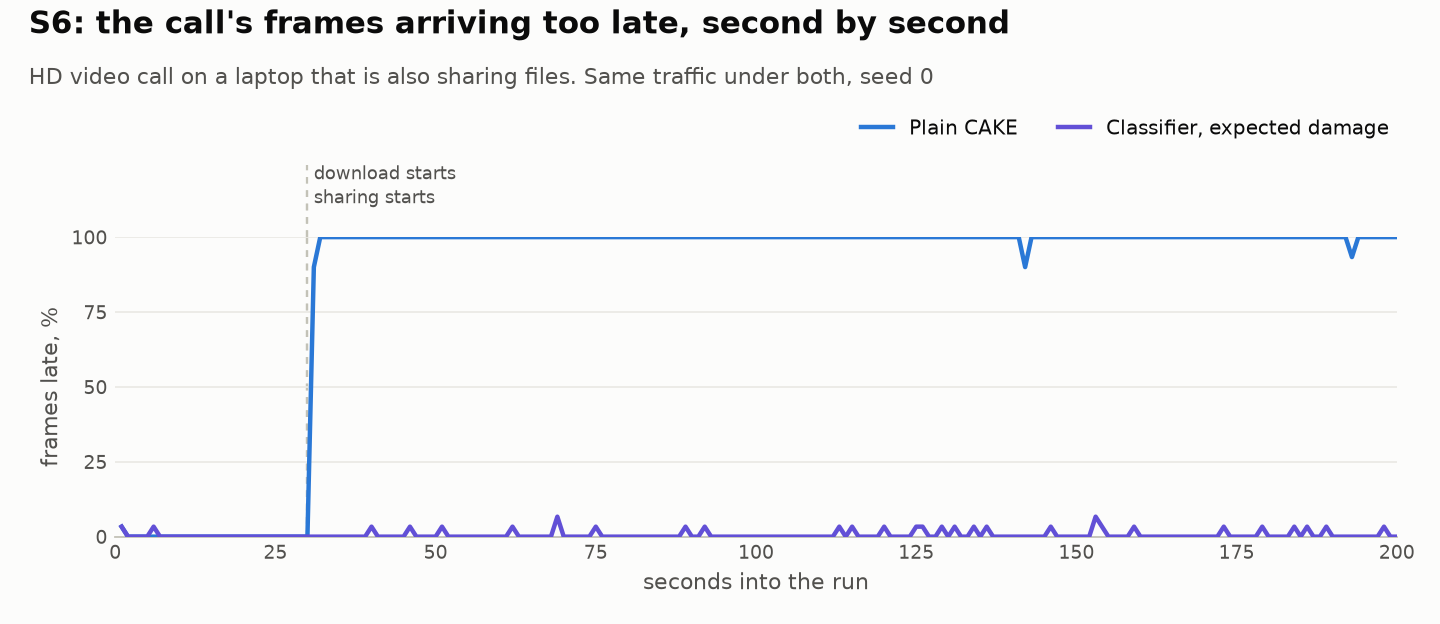
\includegraphics[width=0.49\linewidth]{timeline-S6.png}\hfill
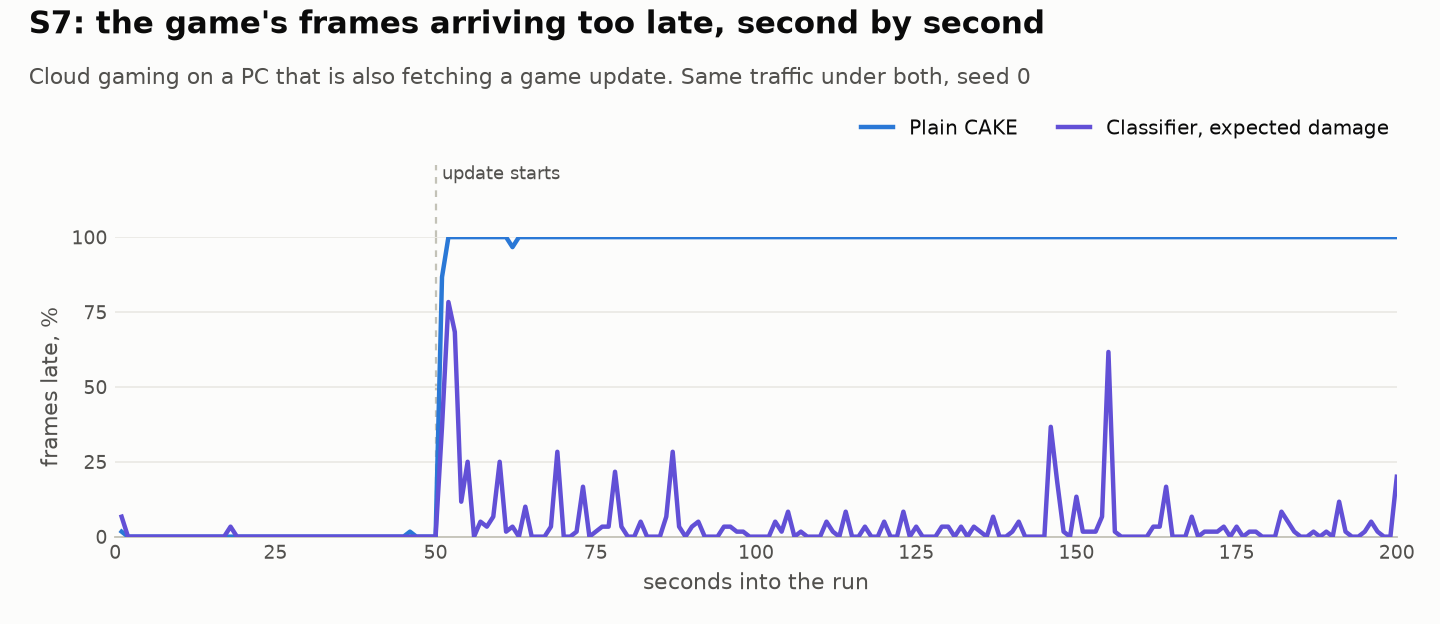
\includegraphics[width=0.49\linewidth]{timeline-S7.png}
\caption{One run each of S6 (left) and S7 (right), second by second. When bulk traffic starts on the same device, plain CAKE lets almost every frame arrive late; AQoSE had already placed the call or game in its tin.}
\end{figure}

Summed over the nine scenarios, the number of flows left unusable is 12.21 with no queue management, 5.54 with plain CAKE, 6.61 with threshold rules, 0.70 with top label and \textbf{0.69 with AQoSE} (medians of ten seeds). The ratio to CAKE depends on the scenario mix and is a summary, not a claim about homes in general. Seed by seed, AQoSE was better than plain CAKE in 49 runs, tied in 41 and worse in none; better than the threshold rules in 52 and tied in 38.

\begin{figure}[H]\centering
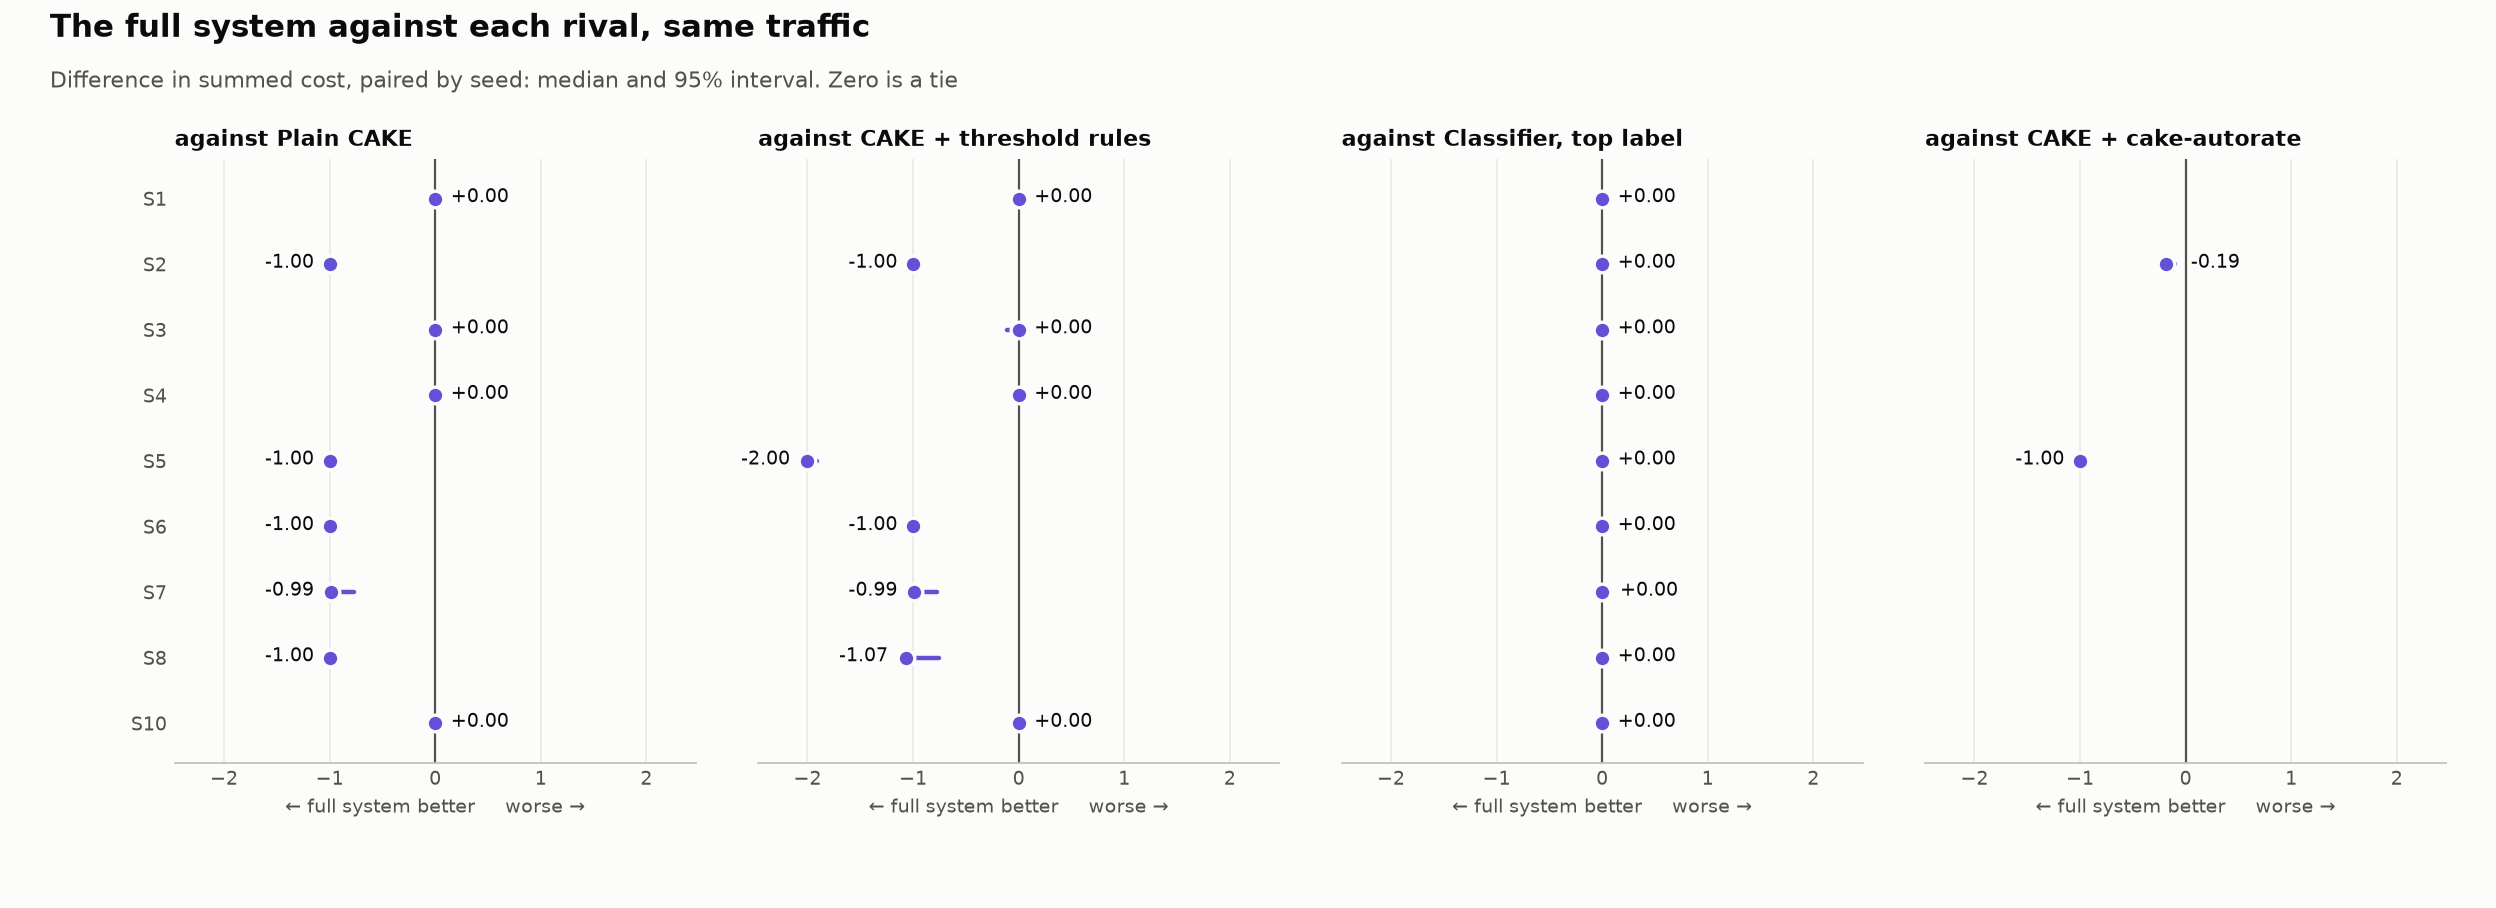
\includegraphics[width=0.92\linewidth]{against-cake.png}
\caption{AQoSE against each rival, paired by seed: median difference in summed cost and 95\% interval. Left of zero AQoSE is better.}
\end{figure}

\paragraph{Against cake-autorate} On S2, where the line slows, cake-autorate cuts late frames from 55.5\% to 4.6\%; AQoSE's built-in estimator reaches 0.9\% with a p95 latency of 19.5\,ms against 95.9\,ms. On S5, where the problem is a call sharing its device with a backup, cake-autorate does nothing (93.3\%), because no rate setting fixes it. AQoSE was better in all 20 paired runs.

\paragraph{Where it ties} In S1, S3, S4 and S10 every interactive flow is alone on its device; CAKE's fairness already protects it, and AQoSE matches CAKE. The damage measurements predicted this before the scenarios ran.

\paragraph{Fail-safe} In all 20 S10 runs, the watchdog restored plain CAKE 2.03 to 2.06\,s after the controller was killed.

\subsection{Fresh seeds and an unseen scenario}
On seeds 10--14, run once, AQoSE was better than plain CAKE in 21 paired runs, tied in 29 and worse in none, and never worse than the threshold rules. The wins held: S6 94.3\% $\to$ 1.0\%, S2 55.5\% $\to$ 0.9\%, S5 78.1\% $\to$ 0.0\%, S7 83.1\% $\to$ 0.4\% late frames (medians). Unusable flows over the ten scenarios: plain CAKE 4.99, threshold rules 7.86, AQoSE 0.99. With five seeds no single comparison reaches significance on its own (Wilcoxon's smallest possible $p$ is 0.0625); the direction agrees on every scenario.

\paragraph{S11} On the scenario written before the freeze and never run during development, plain CAKE already protects everything (0.7\% late frames) and AQoSE ties it (0.0\%); the threshold rules ruin the call (69\%). S11 shows AQoSE stays safe on a home it was not tuned for; it is not a new win over CAKE.

\paragraph{One failure} In one fresh seed of S7 the generator drew a 24.9\,Mbit/s cloud game. AQoSE placed it in Voice, as the taxonomy says, but \texttt{diffserv4} gives the Voice tin priority only up to a quarter of the shaped rate (23.75\,Mbit/s), so the game lost priority and 72\% of its frames were late, no better than plain CAKE. A high-bitrate interactive flow belongs in Video, which has half the rate; this is a design change for the next version.

\subsection{Real calls, replayed}\label{sec:realcall}
Because the testbed's generators are in the model's training data, the live wins might show the classifier recognising its own lab traffic. Two real WhatsApp video calls captured on a home line were therefore replayed packet for packet on a laptop sharing files.

\begin{table}[H]\centering\small
\begin{tabular}{@{}lrrrrr@{}}
\toprule
Late frames (median of 5 seeds) & CAKE & Rules & Top label & \textbf{AQoSE} & AQoSE, v1 model \\
\midrule
S12: call the frozen model never trained on & 57.0\% & 42.7\% & 2.3\% & \ours{2.4\%} & 6.6\% \\
S13: larger call, in the model's training data & 78.7\% & 97.3\% & 14.2\% & \ours{14.4\%} & 30.9\% \\
\bottomrule
\end{tabular}
\caption{The last column uses the model from before the freeze, which never saw WhatsApp at all.}
\end{table}

The frozen model labelled both calls ``video call'' (61--66\% confident) within 0.13\,s in all 20 runs and kept them in Video throughout. The model that never saw WhatsApp labelled them ``voice call'' (91\%), which still protects them, but the reclassifier then moved the calls between Voice and Video several times, which cost quality (6.6\% and 30.9\% late). S13's remaining late frames are almost all on the 4\,Mbit/s upload: the call's real keyframe bursts exceed the half of the link the Video tin may use at priority. The tin was right; the limit is CAKE's share.

\subsection{Is expected damage the reason?}
The classifier, not the decision rule, does most of the work: top label alone takes unusable flows from 5.54 to 0.70, and expected damage to 0.69. To test the decision rule directly, the classifier was weakened by multiplying every input by $\exp(\mathcal{N}(0,\sigma))$.

\begin{table}[H]\centering\small
\begin{tabular}{@{}rrrrrrr@{}}
\toprule
Noise $\sigma$ & Accuracy & \multicolumn{2}{c}{Offline damage} & \multicolumn{2}{c}{S6 call late \%, live} \\
\cmidrule(lr){3-4}\cmidrule(l){5-6}
 & & top label & expected & top label & expected \\
\midrule
0 & 0.976 & 0.302 & 0.235 & 0.7 & 0.5 \\
0.5 & 0.679 & 0.691 & 0.577 & 9.6 & 54.4 \\
1.0 & 0.610 & 0.858 & 0.789 & 62.1 & 94.3 \\
1.5 & 0.551 & 0.915 & 0.863 & 94.1 & 94.3 \\
\bottomrule
\end{tabular}
\caption{Offline, expected damage beats top label at every noise level. Live (three seeds per cell) it did not: with a weaker classifier it left the S6 call worse.}
\end{table}

We therefore do not claim a live benefit for expected damage. It is a principled way to combine uncertain predictions with measured costs, and offline it lowers damage by 20--45\%, but in the live tests its value is as the frame for the guards, not as the source of the wins.

\subsection{Cost}
\begin{table}[H]\centering\small
\begin{tabular}{@{}lr@{}}
\toprule
Component & CPU, \% of one core (mean over scenarios) \\
\midrule
Controller \texttt{aqosd} & 3.6 (3.2--4.4) \\
Classifier service (Go) & 0.04 \\
Delay reflector & 0.22 \\
Watchdog & 0.06 \\
cake-autorate, for comparison & 1.2 (0.8--1.6) \\
\bottomrule
\end{tabular}
\caption{Measured on the reference laptop; a router's processor will show several times these figures.}
\end{table}

%======================================================================
\section{What we learned}
\begin{itemize}
\item \textbf{A tin only matters when the flow has company on its device.} The first damage measurements had each flow alone, and every tin looked alike. That reshaped the scenarios and the claim.
\item \textbf{A wrong label is not a wrong tin.} Calling a video call a voice call harms nothing; both are protected. We measure placements, not only labels.
\item \textbf{The damage table was wrong three times}, each time exposed by a scenario: no reward for demoting a backup beside a call; a call apparently better off in Bulk; Voice rated free for everything.
\item \textbf{Simulations share their author's blind spots.} The capacity estimator passed every simulated test and failed four times on the real testbed; each failure is now a regression test.
\item \textbf{With nothing to go on, do nothing.} Lowering the rate when the probes went silent broke a call on a healthy line; the estimator now holds still.
\item \textbf{Public data is not automatically good data}: each source carries its lab's fingerprint.
\end{itemize}

%======================================================================
\section{Limitations}\label{sec:limits}
\begin{itemize}
\item \textbf{Emulation only.} One laptop, emulated links from 4 to 100\,Mbit/s; no real router, no real home, no Wi-Fi.
\item \textbf{Generated and replayed calls do not adapt.} A real app lowers its bitrate when squeezed; ours lose frames. CAKE's failures are therefore larger here than they would be for real apps.
\item \textbf{Weak across unseen sources.} Leave-one-source-out damage is high; the bulk guard keeps such traffic out of Bulk, but a call can still be left in Best Effort.
\item \textbf{Partly tuned on its own tests.} Seeds 0--9 include those the fixes were found on; the fresh seeds, S11 and the real-call scenarios are the answer, and they are few.
\item \textbf{Thin classes.} 6 voice-call, 8 streaming and 4 large-download flows in the sealed test set.
\item \textbf{The cost scale is self-graded}: the same scale the damage table is built from. The raw measurements (late frames, latency) are the evidence.
\item \textbf{Voice tin share.} A cloud game above a quarter of the line loses priority in Voice (one fresh seed of S7).
\item \textbf{Not measured:} fairness between devices, a flood of short flows, IPv6 end to end, traffic inside a VPN, gigabit rates.
\item \textbf{Leases} take effect at the flow's next window, up to 5\,s, not the 1\,s target.
\end{itemize}

\section{Next steps}
\begin{enumerate}
\item Run on a real OpenWrt router and measure CPU and latency there.
\item Send high-bitrate interactive flows to Video rather than Voice.
\item Add sources per class, especially voice calls and streaming; retrain and check leave-one-source-out.
\item A call generator driven by a real congestion controller, so ``CAKE breaks the call'' becomes ``the call falls to $x$\,kbit/s''.
\item Calm the reclassifier for flows the model is unsure about (the v1 real-call runs).
\end{enumerate}

\section{Conclusion}
A small, calibrated tree model that reads only the headers of a connection's first eight packets is enough to tell CAKE which connection is the call or the game. In emulation, that removes CAKE's one common failure, a call or a game sharing its device with bulk traffic, cuts late frames on real replayed WhatsApp calls from 57\% to 2.4\% and from 79\% to 14\%, ties CAKE everywhere else, and never did worse than the threshold rules existing tools use, at a few percent of one core and with a two-second fall-back to plain CAKE. The next test is a real router in a real home.

\appendix
\section{Reproducing the results}
\begin{verbatim}
make check                      # unit tests, Go and Python
make testbed-check              # tests against the real testbed
make fuzz                       # the safety shield, 5 minutes
scripts/final-runs.sh           # every run after the freeze, then reports
scripts/realcall-runs.sh MAIN WORKTREE  # replayed real calls
python -m aqos_ml.compare \
    --dataset data/dataset/v2.jsonl.gz --final   # sealed test, once
\end{verbatim}
Frozen system: git commit \texttt{4988d91}, model \texttt{lgbm-v2-b3f691d8}, dataset v2 (sha256 \texttt{b3f691d89f00}). Detailed tables, in \texttt{reports/}: \texttt{final.md}, \texttt{fresh.md}, \texttt{realcall.md}, \texttt{realcall-v1.md}, \texttt{ablation.md} and \texttt{head-to-head-v2-test.md}.

\end{document}
